\documentclass[class=scrartcl, 8pt, varwidth=\maxdimen]{standalone}
\usepackage{tikz}
\usepackage{sansmathfonts}
\usepackage[scaled]{helvet}
\let\familydefault\sfdefault
\usepackage[italic]{mathastext}
\usepackage[T1]{fontenc}
\begin{document}
\noindent
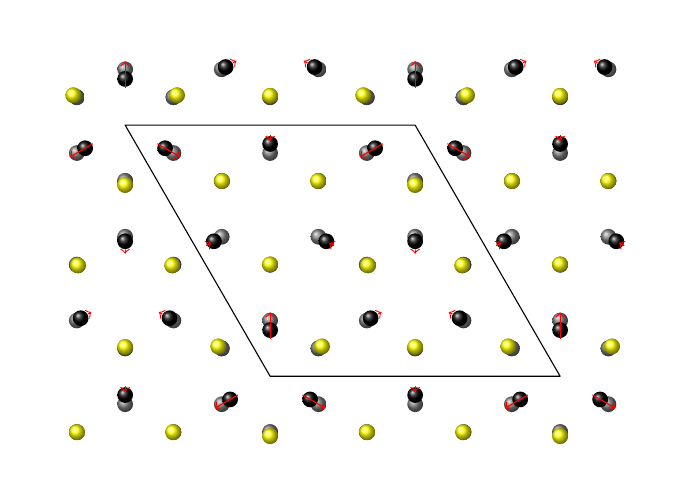
\begin{tikzpicture}[line cap=round, line join=round, mark size=0.05cm]
\useasboundingbox
  (-0.150, -0.150) rectangle +(8.000, 5.665);
\draw plot coordinates {
  (2.929, 1.088) (6.612, 1.088) (4.771, 4.277) (1.088, 4.277)
  (2.929, 1.088) };
\draw [ball color=gray, mark=ball, mark size=1mm, only marks] plot coordinates {
  (1.088, 0.733) (2.315, 0.733) (1.701, 0.379) (1.701, 0.379)
  (0.474, 0.379) (0.474, 0.379) (2.929, 0.379) (2.929, 0.379)
  (1.088, 2.860) (0.474, 1.796) (1.701, 1.796) (0.474, 3.923)
  (1.701, 2.505) (1.701, 2.505) (0.474, 2.505) (0.474, 2.505)
  (1.088, 1.442) (1.088, 1.442) (1.088, 3.569) (1.088, 3.569)
  (2.315, 1.442) (2.315, 1.442) (0.474, 4.632) (0.474, 4.632)
  (4.771, 0.733) (5.999, 0.733) (3.543, 0.733) (5.385, 0.379)
  (5.385, 0.379) (4.157, 0.379) (4.157, 0.379) (6.612, 0.379)
  (6.612, 0.379) (4.771, 2.860) (4.157, 1.796) (5.385, 1.796)
  (2.929, 3.923) (2.315, 2.860) (3.543, 2.860) (4.157, 3.923)
  (1.701, 3.923) (2.929, 1.796) (3.543, 3.569) (3.543, 3.569)
  (2.315, 3.569) (2.315, 3.569) (2.929, 2.505) (2.929, 2.505)
  (5.385, 2.505) (5.385, 2.505) (4.157, 2.505) (4.157, 2.505)
  (4.771, 1.442) (4.771, 1.442) (4.771, 3.569) (4.771, 3.569)
  (3.543, 1.442) (3.543, 1.442) (5.999, 1.442) (5.999, 1.442)
  (2.315, 4.986) (3.543, 4.986) (1.088, 4.986) (2.929, 4.632)
  (2.929, 4.632) (1.701, 4.632) (1.701, 4.632) (4.157, 4.632)
  (4.157, 4.632) (7.226, 0.733) (6.612, 3.923) (5.999, 2.860)
  (7.226, 2.860) (5.385, 3.923) (6.612, 1.796) (7.226, 3.569)
  (7.226, 3.569) (5.999, 3.569) (5.999, 3.569) (6.612, 2.505)
  (6.612, 2.505) (7.226, 1.442) (7.226, 1.442) (5.999, 4.986)
  (7.226, 4.986) (4.771, 4.986) (6.612, 4.632) (6.612, 4.632)
  (5.385, 4.632) (5.385, 4.632) };
\draw [ball color=black, mark=ball, mark size=1mm, only marks] plot coordinates {
  (1.088, 0.849) (2.421, 0.794) (1.088, 2.803) (0.523, 1.825)
  (1.652, 1.825) (0.580, 3.984) (4.771, 0.849) (6.105, 0.794)
  (3.437, 0.794) (4.771, 2.803) (4.206, 1.825) (5.336, 1.825)
  (2.929, 4.038) (2.215, 2.802) (3.643, 2.802) (4.263, 3.984)
  (1.595, 3.984) (2.929, 1.674) (2.364, 5.015) (3.494, 5.015)
  (1.088, 4.864) (7.120, 0.794) (6.612, 4.038) (5.899, 2.802)
  (7.326, 2.802) (5.279, 3.984) (6.612, 1.674) (6.048, 5.015)
  (7.177, 5.015) (4.771, 4.864) };
\draw [ball color=yellow, mark=ball, mark size=1mm, only marks] plot coordinates {
  (1.698, 0.377) (1.698, 0.377) (0.477, 0.377) (0.477, 0.377)
  (2.929, 0.328) (2.929, 0.328) (1.686, 2.496) (1.686, 2.496)
  (0.489, 2.496) (0.489, 2.496) (1.088, 1.460) (1.088, 1.460)
  (1.088, 3.518) (1.088, 3.518) (2.271, 1.467) (2.271, 1.467)
  (0.430, 4.657) (0.430, 4.657) (5.381, 0.377) (5.381, 0.377)
  (4.161, 0.377) (4.161, 0.377) (6.612, 0.328) (6.612, 0.328)
  (3.539, 3.566) (3.539, 3.566) (2.319, 3.566) (2.319, 3.566)
  (2.929, 2.509) (2.929, 2.509) (5.369, 2.496) (5.369, 2.496)
  (4.173, 2.496) (4.173, 2.496) (4.771, 1.460) (4.771, 1.460)
  (4.771, 3.518) (4.771, 3.518) (3.587, 1.467) (3.587, 1.467)
  (5.954, 1.467) (5.954, 1.467) (2.929, 4.650) (2.929, 4.650)
  (1.746, 4.657) (1.746, 4.657) (4.113, 4.657) (4.113, 4.657)
  (7.223, 3.566) (7.223, 3.566) (6.002, 3.566) (6.002, 3.566)
  (6.612, 2.509) (6.612, 2.509) (7.270, 1.467) (7.270, 1.467)
  (6.612, 4.650) (6.612, 4.650) (5.429, 4.657) (5.429, 4.657) };
\draw[draw=red, ->] (1.088, 0.957) -- (1.088, 0.888);
\draw[draw=red, ->] (2.516, 0.849) -- (2.226, 0.682);
\draw[draw=red, ->] (1.088, 2.694) -- (1.088, 2.644);
\draw[draw=red, ->] (0.617, 1.879) -- (0.660, 1.904);
\draw[draw=red, ->] (1.558, 1.879) -- (1.515, 1.904);
\draw[draw=red, ->] (0.674, 4.039) -- (0.385, 3.872);
\draw[draw=red, ->] (4.771, 0.957) -- (4.771, 0.888);
\draw[draw=red, ->] (6.199, 0.849) -- (5.910, 0.682);
\draw[draw=red, ->] (3.343, 0.849) -- (3.632, 0.682);
\draw[draw=red, ->] (4.771, 2.694) -- (4.771, 2.644);
\draw[draw=red, ->] (4.300, 1.879) -- (4.344, 1.904);
\draw[draw=red, ->] (5.241, 1.879) -- (5.198, 1.904);
\draw[draw=red, ->] (2.929, 4.147) -- (2.929, 4.078);
\draw[draw=red, ->] (2.121, 2.748) -- (2.181, 2.782);
\draw[draw=red, ->] (3.737, 2.748) -- (3.677, 2.782);
\draw[draw=red, ->] (4.357, 4.039) -- (4.068, 3.872);
\draw[draw=red, ->] (1.501, 4.039) -- (1.790, 3.872);
\draw[draw=red, ->] (2.929, 1.565) -- (2.929, 1.899);
\draw[draw=red, ->] (2.459, 5.069) -- (2.502, 5.094);
\draw[draw=red, ->] (3.400, 5.069) -- (3.356, 5.094);
\draw[draw=red, ->] (1.088, 4.755) -- (1.088, 5.089);
\draw[draw=red, ->] (7.026, 0.849) -- (7.315, 0.682);
\draw[draw=red, ->] (6.612, 4.147) -- (6.612, 4.078);
\draw[draw=red, ->] (5.804, 2.748) -- (5.865, 2.782);
\draw[draw=red, ->] (7.421, 2.748) -- (7.360, 2.782);
\draw[draw=red, ->] (5.184, 4.039) -- (5.474, 3.872);
\draw[draw=red, ->] (6.612, 1.565) -- (6.612, 1.899);
\draw[draw=red, ->] (6.142, 5.069) -- (6.185, 5.094);
\draw[draw=red, ->] (7.083, 5.069) -- (7.040, 5.094);
\draw[draw=red, ->] (4.771, 4.755) -- (4.771, 5.089);
\end{tikzpicture}%
\end{document}
